\section{Visualization}
\nblink{brats/13\_testnet\_hausdorff\_masks.ipynb}
\nblink{brats/14\_brats\_hausdorff\_masks.ipynb}

To visualize all the distances from the output of the masked image, a new blank image with the same size as the input image is generated. Next, we iterate over all the positions where masks have been
applied to input images. Each position has an associated Hausdorff distance which represents the distance of the output segment generated by the masked image and the ground truth segment.
At each position, we draw a circle with the same diameter as used when generating the mask. The color used to fill this circle represents the Hausdorff distance between the output segment generated by placing a circle at this exact position and the ground truth segment. The color map is scaled to the minimum and maximum Hausdorff distance encountered on all positions.

Figure \ref{hdm_visualization_sample} shows a masked input image (a), (b) shows the baseline output segment from the unchanged image and (c) shows the segment generated by the masked image.
The segment looks completely different from the ground truth, the calculated Hausdorff distance is therefore much bigger than the the distance between the unchanged output segment and the ground truth.

\begin{figure}[H]
    \centering
    \begin{subfigure}{.33\textwidth}
        \centering
        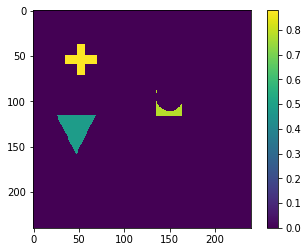
\includegraphics[width=\linewidth]{chapters/06_hdm/visualization/masked.png}
        \caption{Masked input image}
    \end{subfigure}%
    \begin{subfigure}{.33\textwidth}
        \centering
        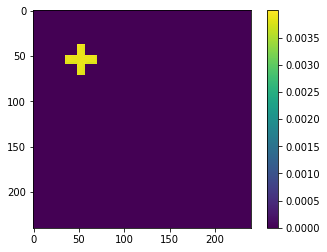
\includegraphics[width=\linewidth]{chapters/06_hdm/visualization/ground_truth.png}
        \caption{Ground truth segment}
    \end{subfigure}
        \begin{subfigure}{.33\textwidth}
        \centering
        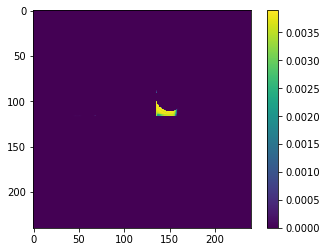
\includegraphics[width=\linewidth]{chapters/06_hdm/visualization/segment.png}
        \caption{Output segment from the masked image}
    \end{subfigure}
    \caption{The output segment (c) from the masked image (a) looks very different than the output segment from the unchanged image (b).}
    \label{hdm_visualization_sample}
\end{figure}

In Figure \ref{hdm_visualization_raw} we see a visualization of all the calculate Hausdorff distances. The dark circle on the upper right corner of the square corresponds to the masked circle from the masked image seen in Figure \ref{hdm_visualization_sample}. The circle is dark because the Hausdorff distance between the output segment (image (c)) and the ground truth (image (b)) is very big. The input image is processed by the canny edge detector and projected on top of the visualization.

To make the visualization interpretable, the original input image should be visible together with the visualization. Do avoid the distortion of the circle colors by projecting
the input image on top of the visualization, we apply the canny edge detector \cite{canny1987computational} on the input image before projecting it on top of the visualization.

\begin{figure}[H]
    \centering
    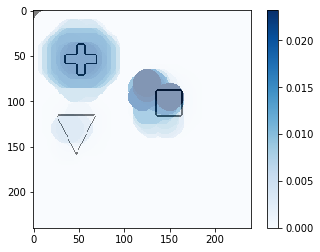
\includegraphics[width=8cm]{chapters/06_hdm/visualization/hdm_raw.png}
    \caption{Hausdorff distance between the left and the right figure: 1353. }
    \label{hdm_visualization_raw}
\end{figure}



\begin{figure}[H]
    \centering
    \begin{subfigure}{.5\textwidth}
        \centering
        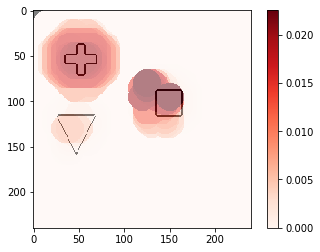
\includegraphics[width=\linewidth]{chapters/06_hdm/visualization/hdm_worse.png}
        \caption{Original shape}
    \end{subfigure}%
    \begin{subfigure}{.5\textwidth}
        \centering
        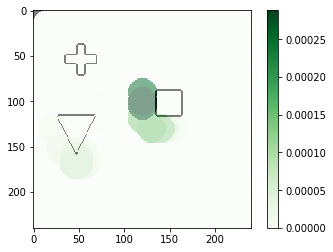
\includegraphics[width=\linewidth]{chapters/06_hdm/visualization/hdm_better.png}
        \caption{Shape moved to the right}
    \end{subfigure}
    \caption{Hausdorff distance between the left and the right figure: 1353. }
    \label{hdm_visualization_better_w}
\end{figure}
